\section{Evidence from published curves, and a diagnostic}
\label{sec:published}

The theory is about a model, not about any particular language model. To ask
whether its one testable prediction, a positive pass@$k$ price, is consistent
with practice, we do not train or run a model: we pass already-published pass@$k$
curves through the diagnostic that the theory defines. The reading is
\emph{indicative}. Published curves are coarse, their values are read from
tables or digitized from plots, and five budgets cannot locate a crossing
precisely. We state every number's source and never claim more than the curve
shows.

\paragraph{The diagnostic.}
The theory turns into a read-off that needs only per-prompt base and RL success
rates, or the pass@$k$ curves they induce, which any evaluation log already
contains. Given base and trained pass@$k$ values, it returns (i) the number of
crossings and their budgets, (ii) the sign-variation bound $\Svar(G)$ of Theorem
\ref{thm:price}(a) and whether it is saturated, (iii) the order-preserving test
of Theorem \ref{thm:price}(d), and (iv) the estimated price, the worst pass@$k$
loss. It ships as a package and a hosted app: paste two columns, get the bound,
the test, and the price. Every user of RLVR has the input on hand, and the
computation adds nothing to a training run, which is the point. We propose that
two numbers be reported alongside pass@1 and pass@$k$: \emph{the price}, the
worst pass@$k$ loss $\max_k(\text{base}-\text{RL})$, and the crossing count.
Both are read from an evaluation log that already exists; reporting them turns
the pass@$k$ reversal from an anecdote into a measured quantity with a bound.

\paragraph{A published case.}
Figure \ref{fig:published} applies the diagnostic to pass@$k$ for Qwen2.5-7B
trained with GRPO on Omni-MATH, as reported by Zhou (2607.20543, Table 2; values
transcribed and to be confirmed against the source). Three readings, all
consistent with the theory:
\begin{itemize}
\item On Omni-MATH the GRPO advantage over base is
$+0.149,+0.144,+0.104,+0.030,-0.008$ at $k=1,4,16,64,256$: it changes sign once,
between $k=64$ and $k=256$. The price is paid, and the single crossing is the
order-preserving regime of Theorem \ref{thm:price}(d).
\item The paper's diversity intervention GRPO+PBA improves on raw GRPO at every
measured $k$, and the frontier explains why. Raw GRPO over-concentrates and sits
\emph{inside} the frontier of Theorem \ref{thm:frontier}, so it is not on the
optimal trade; a diversity bonus moves it toward the frontier, buying both a
higher pass@1 and a later crossing at once. The price versus base is not
removed, only deferred past the measured budget. A bonus helps precisely because
the unconstrained update was suboptimal, which is the frontier's prediction, not
a counterexample to it.
\item On MATH500 neither trained model crosses base for $k\le256$: the price, if
present, lies beyond the measured budget. We claim nothing past $k=256$.
\end{itemize}
This is one dataset read at five budgets, so it is corroboration, not proof. It
shows the predicted structure, a single crossing under GRPO and its delay under a
diversity bonus, in numbers the field already publishes.

\begin{figure}[t]
\centering
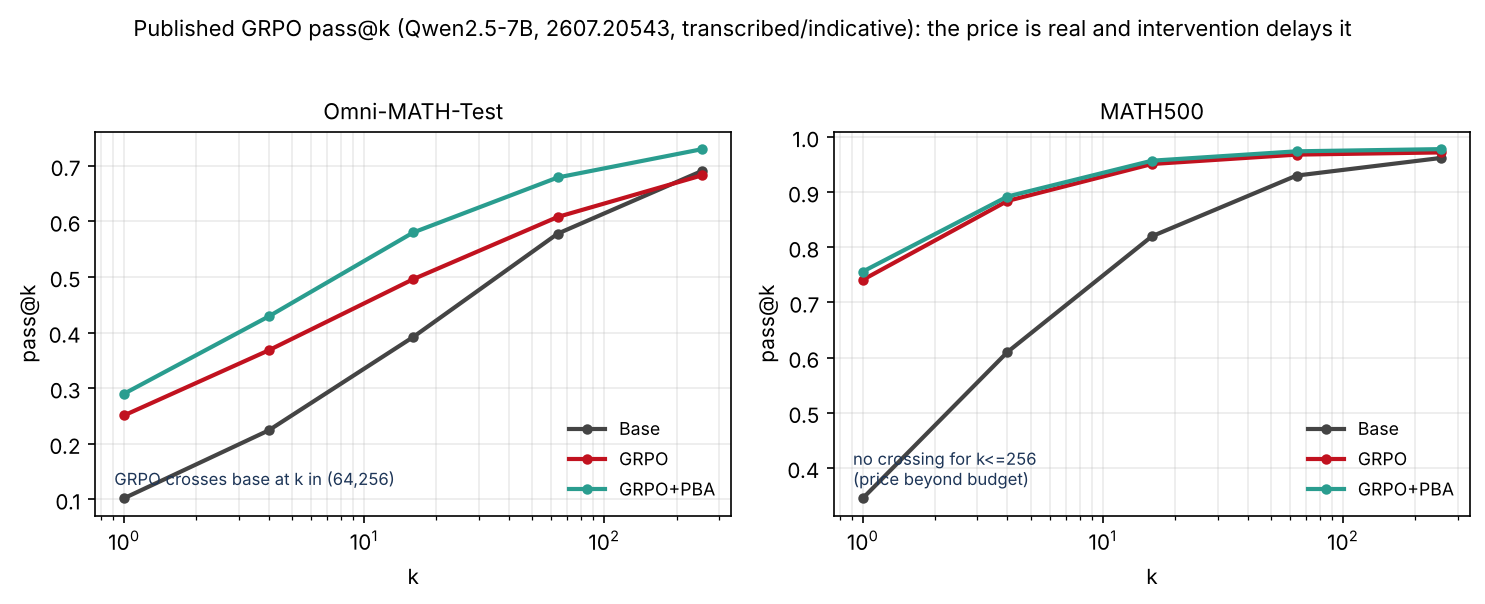
\includegraphics[width=\linewidth]{fig4_published.png}
\caption{Published GRPO pass@$k$ for Qwen2.5-7B (Zhou, 2607.20543, Table 2;
transcribed, indicative). Left, Omni-MATH: GRPO (red) is overtaken by base at the
largest budget, a single crossing, while the diversity intervention GRPO+PBA
(green) stays above through the measured range. Right, MATH500: no crossing for
$k\le256$. The pattern matches the price (Theorem \ref{thm:price}) and the
frontier (Theorem \ref{thm:frontier}); it does not establish behavior beyond the
reported budgets.}
\label{fig:published}
\end{figure}

\paragraph{What would falsify the theory.}
Two statistically supported sign changes in a single base-versus-RL pass@$k$
comparison would exceed $\Svar(G)=1$ only if the shift is not order-preserving;
finding them where the shift is order-preserving would contradict Theorem
\ref{thm:price}(d). A pass@1 gain with no per-prompt loss, under verified
specialization, would contradict Theorem \ref{thm:nfl}. The diagnostic makes both
checks routine on any released evaluation.